% ===============================================================
%  جلسه هشتم
% ===============================================================
\chapter{تساوی‌های آماری، استقلال متغیرهای تصادفی و متغیرهای مخلوط}

\section{مفهوم \lr{almost sure} در آمار و احتمال}

\begin{itemize}
\item در مورد یک \textbf{متغیر یقینی} (\lr{Deterministic}) مانند $A$، راحت می‌توانیم بگوییم $A=2.7$.
\item در مورد یک \textbf{متغیر تصادفی} (\lr{Random}) مانند $X$، عبارت $X=2.7$ معنی خیلی مشخصی می‌دهد: یعنی $\forall\omega\in\Omega$ خواهیم داشت $X(\omega)=2.7$.
\end{itemize}
معمولاً مورد بالا را نمی‌توان به راحتی در مورد یک متغیر تصادفی فهمید، و سطح بالایی از دسترسی (به تک‌تک نقاط $\Omega$) را می‌طلبد. در عوض، چیزی که معمولاً می‌توانیم بفهمیم این است که
\[
\Prob\Big(\big\{\omega\in\Omega\ \big|\ X(\omega)=2.7\big\}\Big)=1,
\]
یعنی متغیر تصادفی $X$ \textbf{با احتمال ۱} مقدار $2.7$ را به خود می‌گیرد.

\begin{definition}[تساوی تقریباً حتمی]
اگر $\Prob(X=c)=1$ باشد می‌گوییم \lr{$X$ almost surely equals to $c$} یا
\[
X\overset{\text{a.s.}}{=}c .
\]
به طور کلی، یک گزاره درباره متغیرهای تصادفی «تقریباً حتماً» (\lr{a.s.}) برقرار است اگر مجموعه $\omega$هایی که در آن‌ها برقرار نیست، احتمال صفر داشته باشد. مثلاً $X\overset{\text{a.s.}}{=}Y$ یعنی $\Prob(X=Y)=1$.
\end{definition}

\begin{itemize}
\item این بدین معنی \textcolor{red!70!black}{\textbf{نیست}} که $X$ \textcolor{red!70!black}{\textbf{نمی‌تواند}} مقداری غیر از $2.7$ را به خود بگیرد. بلکه بدین معنی است که \textcolor{blue!60!black}{\textbf{احتمال آن صفر است}}.
\item یعنی در $N$ آزمایش مستقل برای نمونه‌گیری از $X$، اگر $n(X\neq2.7)$ را تعداد دفعاتی تعریف کنیم که $X$ مقداری غیر از $2.7$ گرفته، آنگاه خواهیم داشت:
\[
\lim_{N\to\infty}\frac{n(X\neq2.7)}{N}=0 .
\]
\item دقت کنید تساوی از حیث \lr{almost sure} \textbf{ضعیف‌تر} از تساوی مطلق است: هر تساوی مطلق، تساوی \lr{a.s.} هم هست، ولی عکس آن لزوماً درست نیست.
\end{itemize}

\begin{example}[تفاوت تساوی مطلق و \lr{a.s.}]
فرض کنید $U\sim\mathrm{Uniform}(0,1)$ و تعریف کنید $X=0$ اگر $U$ گویا باشد و $X=1$ در غیر این صورت. آیا $X=1$؟
\begin{solution}
از نظر مطلق خیر: برای $\omega$هایی که $U(\omega)$ گویاست، $X(\omega)=0$. اما مجموعه اعداد گویای $[0,1]$ شماراست و احتمال هر نقطه برای متغیر پیوسته صفر است؛ پس طبق جمع‌پذیری شمارا $\Prob(U\in\mathbb Q)=\sum_{q}\Prob(U=q)=0$. لذا $\Prob(X=1)=1$ و $X\overset{\text{a.s.}}{=}1$. در عمل هرگز تفاوتی بین $X$ و ثابت ۱ مشاهده نخواهیم کرد.
\end{solution}
\end{example}

\section{استقلال متغیرهای تصادفی}

پیش‌تر \textbf{استقلال آماری} (\lr{Independence}) میان دو رویداد $A,B\in\F$ را تعریف کرده بودیم: $\Prob(A,B)=\Prob(A)\Prob(B)$.

\begin{definition}[استقلال دو متغیر تصادفی]
دو متغیر تصادفی $X,Y$ که روی یک فضای احتمال تعریف شده‌اند را مستقل گوییم، اگر به ازای تمام زیرمجموعه‌های «\textbf{خوبی}» (بورل) از اعداد حقیقی مانند $I_1,I_2\subseteq\R$ داشته باشیم:
\[
\forall I_1,I_2\subseteq\R,\qquad
\begin{array}{l}A\triangleq\{\omega\given X(\omega)\in I_1\}\\ B\triangleq\{\omega\given Y(\omega)\in I_2\}\end{array},\qquad\text{then}\quad A\perp B .
\]
یعنی $\Prob(X\in I_1,\ Y\in I_2)=\Prob(X\in I_1)\Prob(Y\in I_2)$.
\end{definition}

به عبارتی، هر رویدادی در ارتباط با فقط متغیر تصادفی $X$، از هر رویدادی که فقط مرتبط با متغیر تصادفی $Y$ باشد، مستقل باشد.

\begin{note}
\notetitle در عمل کافی است این شرط را برای نیم‌خط‌ها چک کنیم: $X$ و $Y$ مستقل‌اند اگر و تنها اگر برای همه $x,y$:
$\Prob(X\le x,Y\le y)=F_X(x)F_Y(y)$. برای متغیرهای گسسته معادل است با $\Prob(X=x,Y=y)=P_X(x)P_Y(y)$ و برای متغیرهای پیوسته (با چگالی توأم) معادل است با $f_{X,Y}(x,y)=f_X(x)f_Y(y)$ (جلسات بعد).
\end{note}

\section{متغیرهای تصادفی \lr{i.i.d.}}

\begin{definition}[\lr{i.i.d.}]
متغیرهای تصادفی $X_1,X_2,\ldots,X_n$ را در نظر بگیرید. فرض کنید:
\begin{itemize}
\item تمامی این متغیرها از یکدیگر \textbf{مستقل} باشند؛ یعنی هیچ دو زیرمجموعه ناهم‌پوشان از این متغیرها، ارتباطی با دیگری نداشته باشد.
\item توزیع تمام این متغیرها \textbf{یکسان} باشد؛ یعنی $X_1,X_2,\ldots,X_n\sim f_X(x)$.
\end{itemize}
در این صورت به این متغیرها \lr{\textcolor{red!70!black}{i}ndependent and \textcolor{red!70!black}{i}dentically \textcolor{red!70!black}{d}istributed} یا به اختصار \lr{i.i.d.} می‌گوییم.
\end{definition}

مثال کلاسیک: نتایج $n$ پرتاب مستقل یک تاس، یا $n$ نمونه‌ای که از یک «جعبه سیاه» (جلسه ششم) گرفته می‌شود. فرض \lr{i.i.d.} پایه بیشتر روش‌های آماری و یادگیری ماشین است (داده‌های آموزش معمولاً \lr{i.i.d.} فرض می‌شوند).

\begin{warning}
\warntitle دقت کنید که دو متغیر تصادفی می‌توانند اصلاً مستقل نباشند (تقریباً هیچ دو متغیر تصادفی واقعی در جهان مستقل نیستند!). «هم‌توزیع بودن» و «مستقل بودن» دو مفهوم کاملاً جدا هستند:
\begin{itemize}
\item مثلاً فرض کنید $X\sim\lambda e^{-\lambda x}u(x)$ توزیع نمایی داشته، و متغیر تصادفی $Y\sim\mathcal N(0,1)$ توزیع نرمال استاندارد داشته باشد. اما دانستن مقدار $X$، یا اطلاعاتی در مورد آن، باعث شود توزیع $Y$ تغییر کند. این دو هم‌توزیع نیستند و مستقل هم نیستند.
\item از سوی دیگر، این بار فرض کنید $X,Y\sim\mathcal N(0,1)$، یعنی \textbf{هم‌توزیع} باشند. با این اطلاعات در مورد ارتباط این دو با یکدیگر حرفی نمی‌توان زد. هم می‌توانیم داشته باشیم $X\perp Y$، و هم می‌توانیم داشته باشیم $X\overset{\text{a.s.}}{=}Y$ (یا حتی $Y=-X$ که آن هم $\mathcal N(0,1)$ است!).
\end{itemize}
\end{warning}

\section{رفتار دُم توزیع‌های مختلف \lr{(Tail Behavior of Various Distributions)}}

در این بخش، برای هر توزیع یک نمونه ۱۰۰۰تایی \lr{i.i.d.} تولید کرده‌ایم و مقادیر نمونه‌ها را بر حسب شماره نمونه رسم کرده‌ایم. سؤال این است: \emph{با نگاه به نمونه‌ها، می‌توان حدس زد از کدام توزیع آمده‌اند؟} ویژگی مهمی که در این نمودارها دیده می‌شود، «\textbf{دُم}» (\lr{tail}) توزیع است؛ یعنی اینکه احتمال مقادیر بسیار بزرگ با چه سرعتی کم می‌شود.

\newcommand{\sampplot}[4]{%
\begin{center}
\begin{tikzpicture}
\begin{axis}[width=14cm,height=4.6cm,xmin=1,xmax=1000,ymin=#2,ymax=#3,xlabel={\lr{Sample Index}},ylabel={\lr{Sample Value}},grid=major,grid style={gray!20},tick label style={font=\scriptsize}]
\addplot[blue,thin,mark=*,mark size=0.5pt] table[x=i,y=x]{data/samp_#1.dat};
\draw[black] (axis cs:1,0) -- (axis cs:1000,0);
\end{axis}
\end{tikzpicture}\\[-1mm]
{\small #4}
\end{center}}

\subsection{نمونه اول}
\sampplot{unif}{-0.7}{1.7}{نمونه‌ها همگی بین ۰ و ۱ هستند و به طور یکنواخت پخش شده‌اند.}
\textbf{جواب:} توزیع یکنواخت $X\sim\frac{\ind(a\le X\le b)}{b-a}$، در اینجا $\mathrm{Uniform}(0,1)$. دقت کنید تمام نمونه‌ها بین ۰ و ۱ هستند؛ این توزیع اصلاً دُم ندارد (تکیه‌گاه آن کران‌دار است).

\subsection{نمونه دوم}
\sampplot{gauss}{-5}{5}{نمونه‌ها حول صفر متمرکزند و هر از گاهی مقادیر بزرگ‌تر (تا حدود $\pm3$) دیده می‌شوند.}
\textbf{جواب:} توزیع گاوسی $X\sim\frac{1}{\sqrt{2\pi}\sigma}e^{-\frac{(x-\mu)^2}{2\sigma^2}}$، در اینجا $\mathcal N(0,1)$: هر از گاهی نمونه‌های بزرگ درست می‌شوند، ولی کماکان متمرکز هستند. طبق قاعده «۶۸، ۹۵ و ۹۹٫۷ درصد»، تقریباً همه نمونه‌ها در بازه $[-3,3]$ می‌افتند؛ در ۱۰۰۰ نمونه انتظار داریم فقط حدود ۳ نمونه بیرون از این بازه باشند.

\subsection{نمونه سوم}
\sampplot{expo}{-1}{9}{نمونه‌ها همگی نامنفی هستند و گاهی مقادیر بزرگ (تا حدود ۸) ظاهر می‌شوند.}
\textbf{جواب:} توزیع نمایی $X\sim\lambda e^{-\lambda x}u(x)$، در اینجا $\mathrm{Exp}(\lambda=1)$. برخلاف توزیع گاوسی که چگالی دم آن $e^{-O(x^2)}$ است، دم نمایی از قدر مرتبه $e^{-O(x)}$ است و لذا \lr{spike}های بزرگ بیشتر مشاهده می‌شوند. مثلاً $\Prob(X>5)=e^{-5}\approx0.0067$ (حدود ۷ نمونه از ۱۰۰۰)، در حالی که برای گاوسی استاندارد $\Prob(Z>5)\approx3\times10^{-7}$.

\subsection{نمونه چهارم}
\sampplot{cauchy}{-70}{70}{(مقادیر برای نمایش در بازه $\pm70$ بریده شده‌اند.) و اما مورد آخر\ldots\ حدس شما چیست؟ چه چیزی در مورد این توزیع عجیب است؟}
\textbf{جواب:} توزیع کوشی
\[
X\sim\frac{1}{\pi(1+x^2)},
\]
در اینجا $\mathrm{Cauchy}(0,1)$. چگالی دم این توزیع $O(1/x^2)$ است، و یکی از قوی‌دم‌ترین (\lr{heavy-tail}) توزیع‌های دنیا محسوب می‌شود. لطفاً به \lr{Spike}های آن دقت کنید! بیشتر نمونه‌ها نزدیک صفرند اما هر از گاهی مقادیری در حد ده‌ها یا صدها ظاهر می‌شوند.

\begin{note}
\notetitle \textbf{چه چیزی عجیب است؟} برای کوشی، $\Prob(|X|>t)=1-\frac2\pi\arctan t\approx\frac{2}{\pi t}$؛ یعنی احتمال مقادیر بزرگ فقط به صورت $1/t$ کم می‌شود. مثلاً $\Prob(|X|>60)\approx0.0106$، پس در ۱۰۰۰ نمونه حدود ۱۰ نمونه بزرگ‌تر از ۶۰ (از نظر قدر مطلق) خواهیم داشت! نتیجه عجیب‌تر (که در جلسات بعد می‌بینیم): این توزیع \textbf{میانگین ندارد} ــ انتگرال $\int|x|\frac{1}{\pi(1+x^2)}\dd x$ واگراست ــ و میانگین نمونه‌ای $\frac1n\sum X_i$ هیچ‌گاه همگرا نمی‌شود (در واقع خودش دوباره کوشی استاندارد است!).
\end{note}

\begin{center}
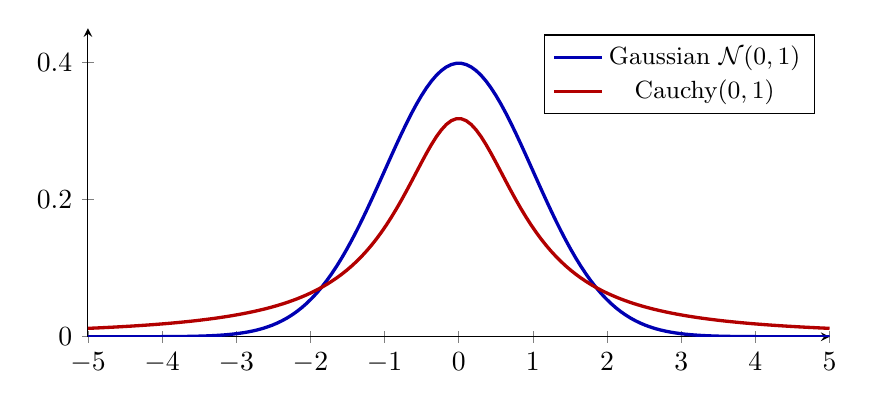
\begin{tikzpicture}
\begin{axis}[width=11cm,height=5.5cm,axis lines=left,xmin=-5,xmax=5,ymin=0,ymax=0.45,samples=150,domain=-5:5,legend style={font=\small}]
\addplot[blue!70!black,very thick] {exp(-x^2/2)/sqrt(2*pi)}; \addlegendentry{\lr{Gaussian $\mathcal N(0,1)$}}
\addplot[red!70!black,very thick] {1/(pi*(1+x^2))}; \addlegendentry{\lr{Cauchy$(0,1)$}}
\end{axis}
\end{tikzpicture}
\end{center}

\section{متغیرهای تصادفی مخلوط (گسسته و پیوسته)}

\begin{example}[دماسنج نامطمئن]
فرض کنید قصد داریم تا دمای یک محیط را با یک دماسنج دیجیتال نامطمئن اندازه‌گیری کنیم:
\begin{itemize}
\item در هر بار اندازه‌گیری، دماسنج با احتمال موفقیت $p$ کار کرده و خروجی آن به شکل یک توزیع گاوسی (با انحراف معیار $\sigma$) حول دمای واقعی (که با $\mu$ نشان داده می‌شود) ظاهر می‌گردد.
\item اما دماسنج با احتمال $1-p$ کار نکرده و دمای پیش‌فرض «$\mu'$» را نشان خواهد داد.
\end{itemize}
\textbf{سؤال:} در صورتی که عدد خروجی دماسنج را با متغیر تصادفی $X$ نشان دهیم، توزیع آن را بیابید.
\end{example}

\begin{center}
\begin{tikzpicture}[>=Stealth]
\node[draw,rounded corners,fill=gray!10,minimum width=2.6cm,minimum height=0.9cm] (T) at (0,0) {دماسنج};
\node[draw,thick,minimum height=0.8cm] (G) at (-3,-2.2) {$\mathcal N(\mu,\sigma^2)$};
\node[draw,thick,minimum height=0.8cm,minimum width=1.2cm] (M) at (3,-2.2) {$\mu'$};
\draw[->,thick] (T) -- node[above left]{$p$} (G);
\draw[->,thick] (T) -- node[above right]{$1-p$} (M);
\end{tikzpicture}
\end{center}

ابتدا \lr{CDF} را با قانون احتمال کل می‌نویسیم ($W$ = «دماسنج کار کند»):
\[
F_X(x)=\Prob(X\le x\given W)\Prob(W)+\Prob(X\le x\given W^c)\Prob(W^c)
=p\,\Phi\Big(\frac{x-\mu}{\sigma}\Big)+(1-p)\,\ind(x\ge\mu').
\]
این \lr{CDF} در نقطه $\mu'$ یک \textbf{پرش} به اندازه $1-p$ دارد و در بقیه جاها هموار است. پس $X$ نه گسسته است و نه پیوسته؛ یک متغیر \textbf{مخلوط} است. اما مشتق تابع پله در نقطه پرش چیست؟ برای پاسخ، به یک ابزار ریاضی نیاز داریم.

\subsection{تابع دلتای دیراک}
در ریاضیات کاربردی، موارد بسیاری وجود خواهند داشت که در آنان به دنبال \textbf{توابعی} می‌گردیم که تنها در \textbf{یک نقطه} غیر صفر شوند. در عین حال، نیاز داریم تا انتگرال تابع فوق در هر بازه‌ای که شامل نقطه مورد نظر است مقداری غیرصفر داشته باشد. به یکی از توابع معروفی که خواص فوق را دارد، \textbf{تابع دلتای دیراک} $\delta(x)$ اطلاق می‌گردد:
\[
\delta(x)=\begin{cases}+\infty & x=0\\ 0 & x\neq0\end{cases},
\qquad\qquad
\int_R\delta(x)\dd x=\begin{cases}1 & 0\in R\\ 0 & 0\notin R\end{cases}.
\]

\begin{itemize}
\item در ریاضیات محض و شاخه آنالیز حقیقی، می‌توان نشان داد که موجودی مانند \textbf{دلتای دیراک} $\delta(x)$ نمی‌تواند یک تابع انتگرال‌پذیر (به معنای معمول) باشد: تابعی که جز در یک نقطه صفر است، انتگرال صفر دارد.
\item در واقع، انتگرال مفاهیمی مانند دلتای دیراک به صورت اختصاصی و جداگانه تعریف می‌شوند (تعریف عام \textbf{جمع ریمان} یا \lr{\textbf{Riemann Sum}} در مورد دلتای دیراک برقرار نیست). در ریاضیات دقیق، $\delta$ یک «تابع تعمیم‌یافته» یا \lr{distribution} است.
\end{itemize}

\textbf{چگونگی ساختن تابع دلتای دیراک:} دلتا را می‌توان حد دنباله‌ای از توابع معمولی با مساحت ۱ در نظر گرفت که هر چه باریک‌تر و بلندتر می‌شوند:
\begin{itemize}
\item پالس مستطیلی به عرض $\varepsilon$ و ارتفاع $\frac1\varepsilon$ حول صفر، وقتی $\varepsilon\to0$؛
\item چگالی گاوسی $\frac{1}{\sqrt{4\pi\alpha}}e^{-x^2/(4\alpha)}$ (یعنی $\mathcal N(0,2\alpha)$)، وقتی $\alpha\to0$.
\end{itemize}

\begin{center}
\begin{tikzpicture}
\begin{axis}[width=7cm,height=5cm,axis lines=middle,xmin=-2,xmax=2,ymin=0,ymax=4.5,xtick=\empty,ytick=\empty,samples=200,domain=-2:2,title={\small پالس‌های مستطیلی}]
\addplot[blue,thick,const plot] coordinates {(-2,0) (-0.5,0) (-0.5,1) (0.5,1) (0.5,0) (2,0)};
\addplot[red,thick,const plot] coordinates {(-2,0) (-0.25,0) (-0.25,2) (0.25,2) (0.25,0) (2,0)};
\addplot[green!50!black,thick,const plot] coordinates {(-2,0) (-0.125,0) (-0.125,4) (0.125,4) (0.125,0) (2,0)};
\end{axis}
\end{tikzpicture}
\begin{tikzpicture}
\begin{axis}[width=7cm,height=5cm,axis lines=middle,xmin=-3,xmax=3,ymin=0,ymax=1,xtick=\empty,ytick=\empty,samples=200,domain=-3:3,title={\small چگالی‌های گاوسی}]
\addplot[blue,thick] {exp(-x^2/(4*2.5))/sqrt(4*pi*2.5)};
\addplot[red,thick] {exp(-x^2/(4*0.5))/sqrt(4*pi*0.5)};
\addplot[green!50!black,thick] {exp(-x^2/(4*0.1))/sqrt(4*pi*0.1)};
\end{axis}
\end{tikzpicture}
\end{center}

\begin{theorem}[خاصیت غربالی]
برای هر تابع پیوسته $g$:
$\displaystyle\int_{-\infty}^{\infty}g(x)\,\delta(x-a)\dd x=g(a)$. همچنین $\delta(x)=\frac{\dd}{\dd x}u(x)$ که $u$ تابع پله واحد است (به این معنا که $\int_{-\infty}^x\delta(t)\dd t=u(x)$).
\end{theorem}

\subsection{حل مسئله دماسنج نامطمئن}
با مشتق‌گیری از \lr{CDF} و استفاده از $\frac{\dd}{\dd x}\ind(x\ge\mu')=\delta(x-\mu')$:
\[
\boxed{\ f_X(x)=\frac{p}{\sqrt{2\pi}\sigma}e^{-\frac{(x-\mu)^2}{2\sigma^2}}+(1-p)\,\delta(x-\mu')\ }
\]
این \lr{PDF} یک «زنگوله» با مساحت $p$ به‌علاوه یک «ضربه» با وزن $1-p$ در نقطه $\mu'$ است؛ مساحت کل $p+(1-p)=1$.

\begin{center}
\begin{tikzpicture}
\begin{axis}[width=10cm,height=5cm,axis lines=left,xmin=0,xmax=10,ymin=0,ymax=0.45,xtick={2,6},xticklabels={$\mu'$,$\mu$},ytick=\empty,samples=150,domain=0:10]
\addplot[blue,very thick] {0.7*exp(-(x-6)^2/2)/sqrt(2*pi)};
\draw[-{Stealth},very thick,red] (axis cs:2,0) -- (axis cs:2,0.4) node[right,font=\small]{$(1-p)\,\delta(x-\mu')$};
\node[blue,font=\small] at (axis cs:8.3,0.25) {$p\,\mathcal N(\mu,\sigma^2)$};
\end{axis}
\end{tikzpicture}
\end{center}

\subsection{تبدیل \lr{PMF} به \lr{PDF}}
با دلتای دیراک، متغیرهای گسسته را هم می‌توان با \lr{PDF} توصیف کرد. فرض کنید که متغیر تصادفی گسسته $X$ دارای تابع جرم احتمال به شکل زیر است:
\[
P(X=x_i)=p_i,\qquad\forall x_i\in\mathrm{Support}(X).
\]
در این صورت، تابع چگالی احتمال (\lr{PDF}) این متغیر تصادفی به شکل زیر خواهد بود:
\[
f_X(x)=\sum_ip_i\,\delta(x-x_i).
\]
بدین ترتیب یک چارچوب واحد برای همه متغیرها (گسسته، پیوسته و مخلوط) داریم: احتمال هر بازه برابر انتگرال \lr{PDF} روی آن است، به شرطی که ضربه‌های داخل بازه را نیز در نظر بگیریم.

\section{تمرین‌های تکمیلی}

\begin{exercise}
در مسئله دماسنج نامطمئن با $\mu=25$، $\sigma=1$، $\mu'=0$ و $p=0.9$، احتمال اینکه دماسنج عددی بین ۲۴ و ۲۶ نشان دهد چقدر است؟ احتمال اینکه دقیقاً صفر نشان دهد چطور؟
\end{exercise}
\begin{solution}
$P(24\le X\le26)=0.9\times P(|Z|\le1)+0.1\times\ind(0\in[24,26])\approx0.9\times0.683=0.615$.
و $P(X=0)=1-p=0.1$ (وزن ضربه در صفر؛ بخش گاوسی در یک نقطه احتمال صفر دارد).
\end{solution}

\begin{exercise}
دو متغیر $X,Y\in\{0,1\}$ با جدول توأم زیر داده شده‌اند: $P(0,0)=0.3$، $P(0,1)=0.2$، $P(1,0)=0.3$، $P(1,1)=0.2$. آیا $X$ و $Y$ مستقل‌اند؟ آیا هم‌توزیع‌اند؟
\end{exercise}
\begin{solution}
حاشیه‌ها: $P_X(0)=0.5$، $P_X(1)=0.5$، $P_Y(0)=0.6$، $P_Y(1)=0.4$. حاصل‌ضرب‌ها: $0.5\times0.6=0.3$ و $0.5\times0.4=0.2$؛ همه خانه‌ها برابرند، پس \textbf{مستقل‌اند}. اما توزیع حاشیه‌ای‌شان متفاوت است، پس \textbf{هم‌توزیع نیستند} (و \lr{i.i.d.} نیستند).
\end{solution}

\begin{exercise}
\lr{PDF} متغیر $X$ = «تعداد شیرها در دو پرتاب سکه سالم» را با دلتای دیراک بنویسید و $\int_{0.5}^{3}f_X(x)\dd x$ را حساب کنید.
\end{exercise}
\begin{solution}
$f_X(x)=\frac14\delta(x)+\frac12\delta(x-1)+\frac14\delta(x-2)$. بازه $[0.5,3]$ شامل نقاط ۱ و ۲ است؛ پس انتگرال برابر $\frac12+\frac14=\frac34=P(X\ge1)$ است.
\end{solution}
